\section{Phân hệ Xác thực Người dùng (Auth)}

\subsection{Đặc tả Use Case}
Phân hệ Xác thực quản lý vòng đời tài khoản của người dùng, cung cấp cơ chế đăng ký và đăng nhập bảo mật bằng JSON Web Token (JWT). Sơ đồ Use Case được minh họa tại Hình~\ref{fig:usecase-auth}.

\begin{figure}[htbp]
    \centering
    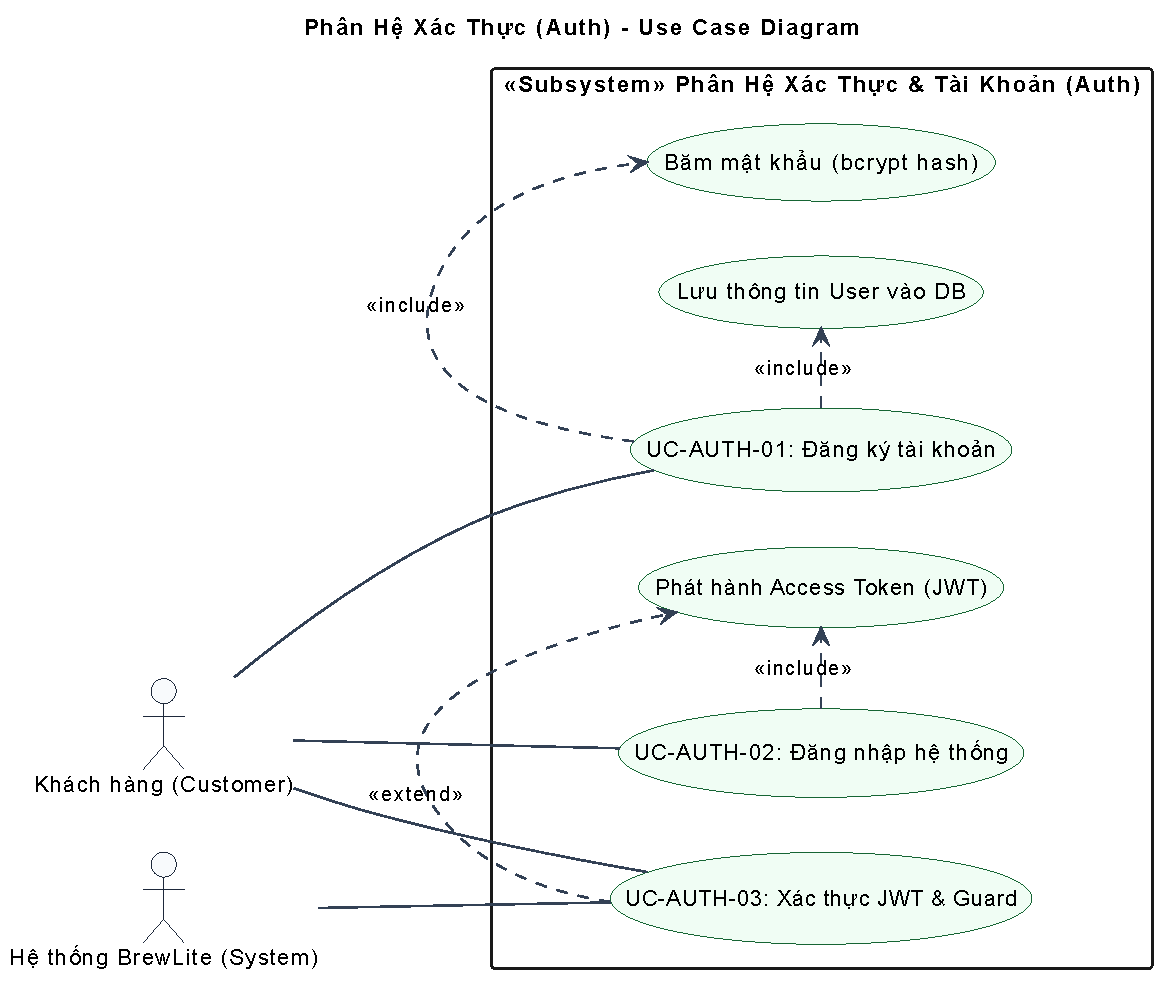
\includegraphics[width=0.75\textwidth]{figures/usecase-auth.pdf}
    \caption{Sơ đồ Use Case - Phân hệ Xác thực}
    \label{fig:usecase-auth}
\end{figure}

\begin{table}[htbp]
\centering
\small
\caption{Đặc tả Use Case: Đăng ký và Đăng nhập người dùng}
\label{tab:uc-spec-auth}
\begin{tabularx}{\textwidth}{p{2.3cm}XX}
\toprule
\textbf{Mục} & \textbf{Đăng ký (UC-AUTH-01)} & \textbf{Đăng nhập (UC-AUTH-02)} \\
\midrule
\textbf{Actor} & Khách vãng lai (Guest) & Khách hàng đã có tài khoản \\
\midrule
\textbf{Tiền điều kiện} & Chưa đăng nhập; địa chỉ email chưa tồn tại trên hệ thống. & Đã có tài khoản trên hệ thống; tài khoản ở trạng thái hoạt động. \\
\midrule
\textbf{Hậu điều kiện} & Bản ghi mới được tạo trong bảng \texttt{users}; mật khẩu được băm Bcrypt 10 rounds; khởi tạo 0 điểm loyalty. & Cấp phát mã thông báo JWT \texttt{accessToken}; lưu trữ tại client để xác thực các request kế tiếp. \\
\midrule
\textbf{Luồng chính} & 
1. Người dùng nhập email, mật khẩu (\(\ge\) 6 ký tự), họ tên.\newline
2. Nhấn "Đăng ký".\newline
3. Hệ thống kiểm tra hợp lệ DTO và tính duy nhất của email.\newline
4. Băm mật khẩu bằng \texttt{bcrypt.hash(password, 10)}.\newline
5. Tạo người dùng trong DB và trả về thông tin (loại trừ \texttt{password\_hash}). & 
1. Người dùng nhập email và mật khẩu.\newline
2. Nhấn "Đăng nhập".\newline
3. Hệ thống tìm người dùng theo email.\newline
4. So sánh mật khẩu bằng \texttt{bcrypt.compare(password, hash)}.\newline
5. Sinh mã JWT chứa payload \texttt{\{sub, email\}}.\newline
6. Trả về token và thông tin hồ sơ người dùng. \\
\midrule
\textbf{Luồng ngoại lệ} & 
- DTO không hợp lệ: Trả về mã \texttt{400 Bad Request}.\newline
- Trùng email: Trả về \texttt{409 Conflict} ("Email đã được sử dụng"). & 
- Email không tồn tại hoặc sai mật khẩu: Trả về \texttt{401 Unauthorized} ("Email hoặc mật khẩu không chính xác"). \\
\bottomrule
\end{tabularx}
\end{table}

\subsection{Sơ đồ Hoạt động (Activity Diagram)}
Sơ đồ Hoạt động mô tả chi tiết quy trình xử lý luồng đăng nhập và kiểm tra xác thực người dùng được biểu diễn tại Hình~\ref{fig:activity-auth}.

\begin{figure}[htbp]
    \centering
    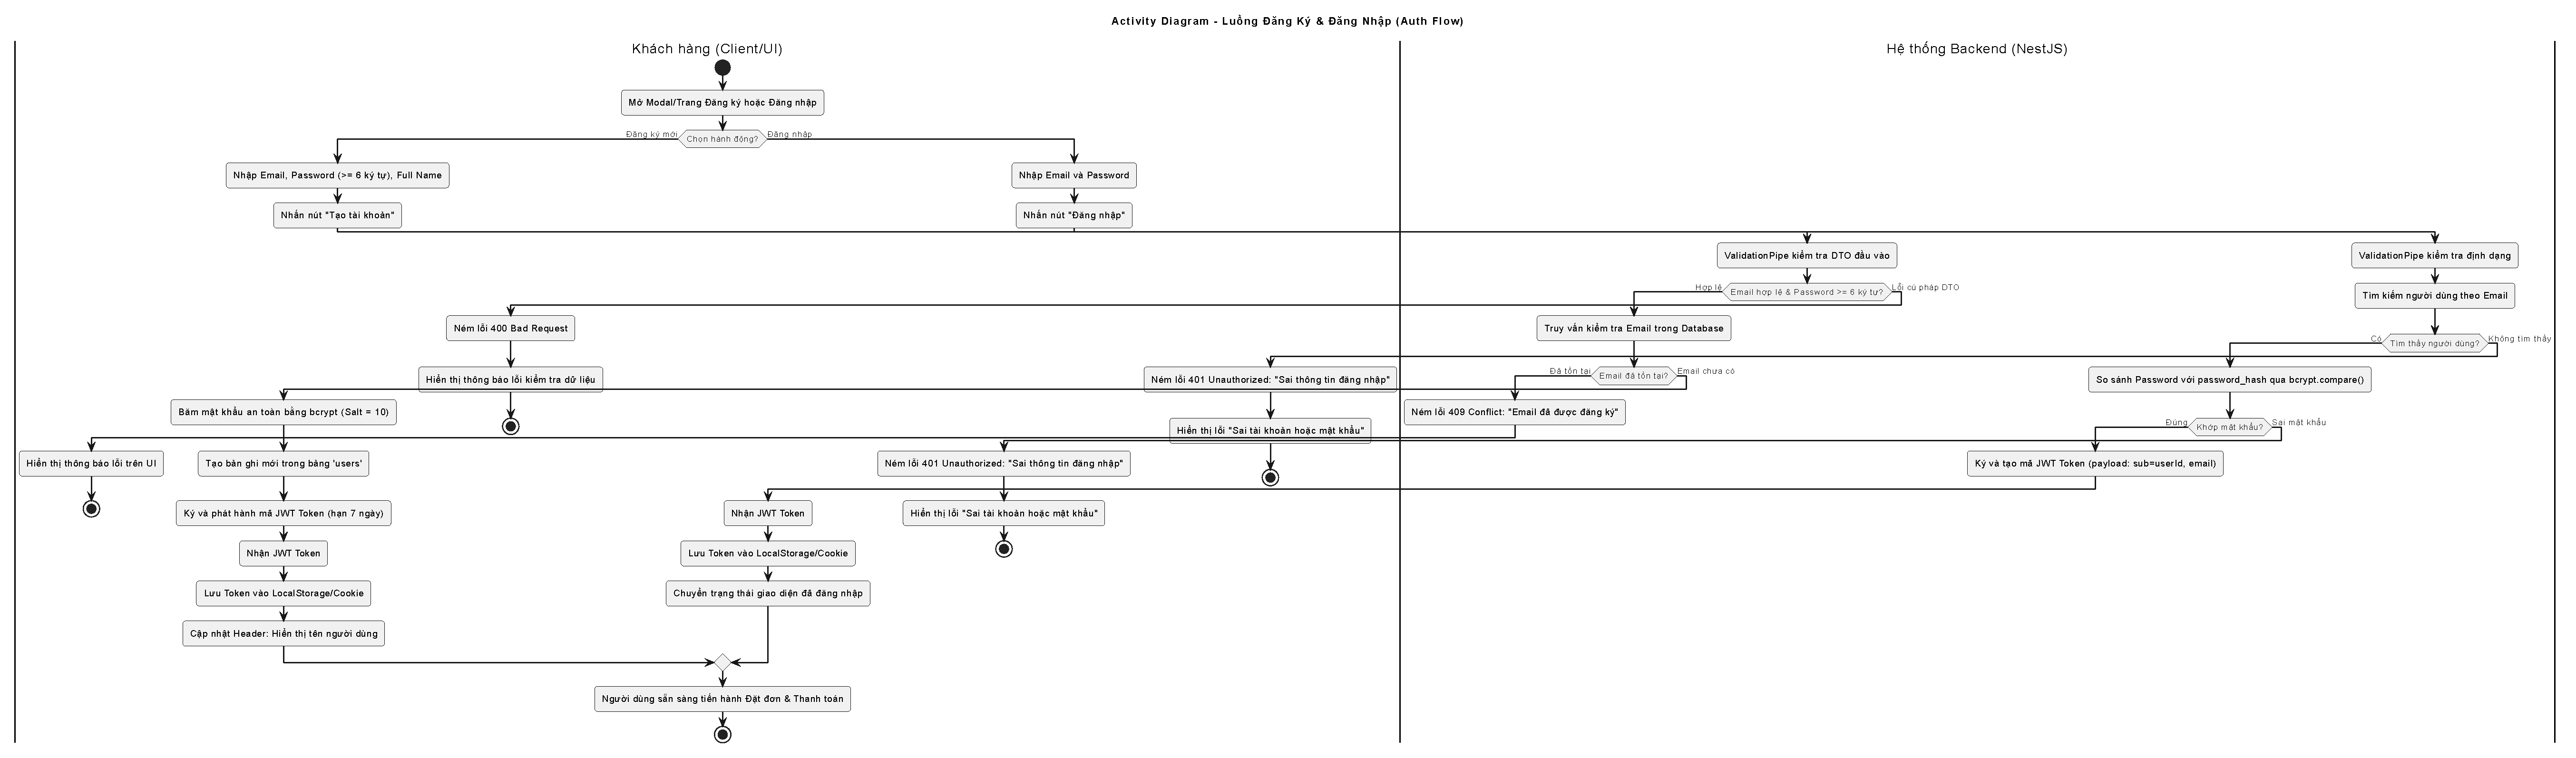
\includegraphics[width=0.75\textwidth]{figures/activity-auth.pdf}
    \caption{Sơ đồ Hoạt động - Phân hệ Xác thực}
    \label{fig:activity-auth}
\end{figure}

\subsection{Sơ đồ Tuần tự (Sequence Diagram)}
Sơ đồ Tuần tự phản ánh chuẩn xác các lời gọi hàm từ giao diện qua Controller đến Service và Prisma DB tại Hình~\ref{fig:sequence-auth}.

\begin{figure}[htbp]
    \centering
    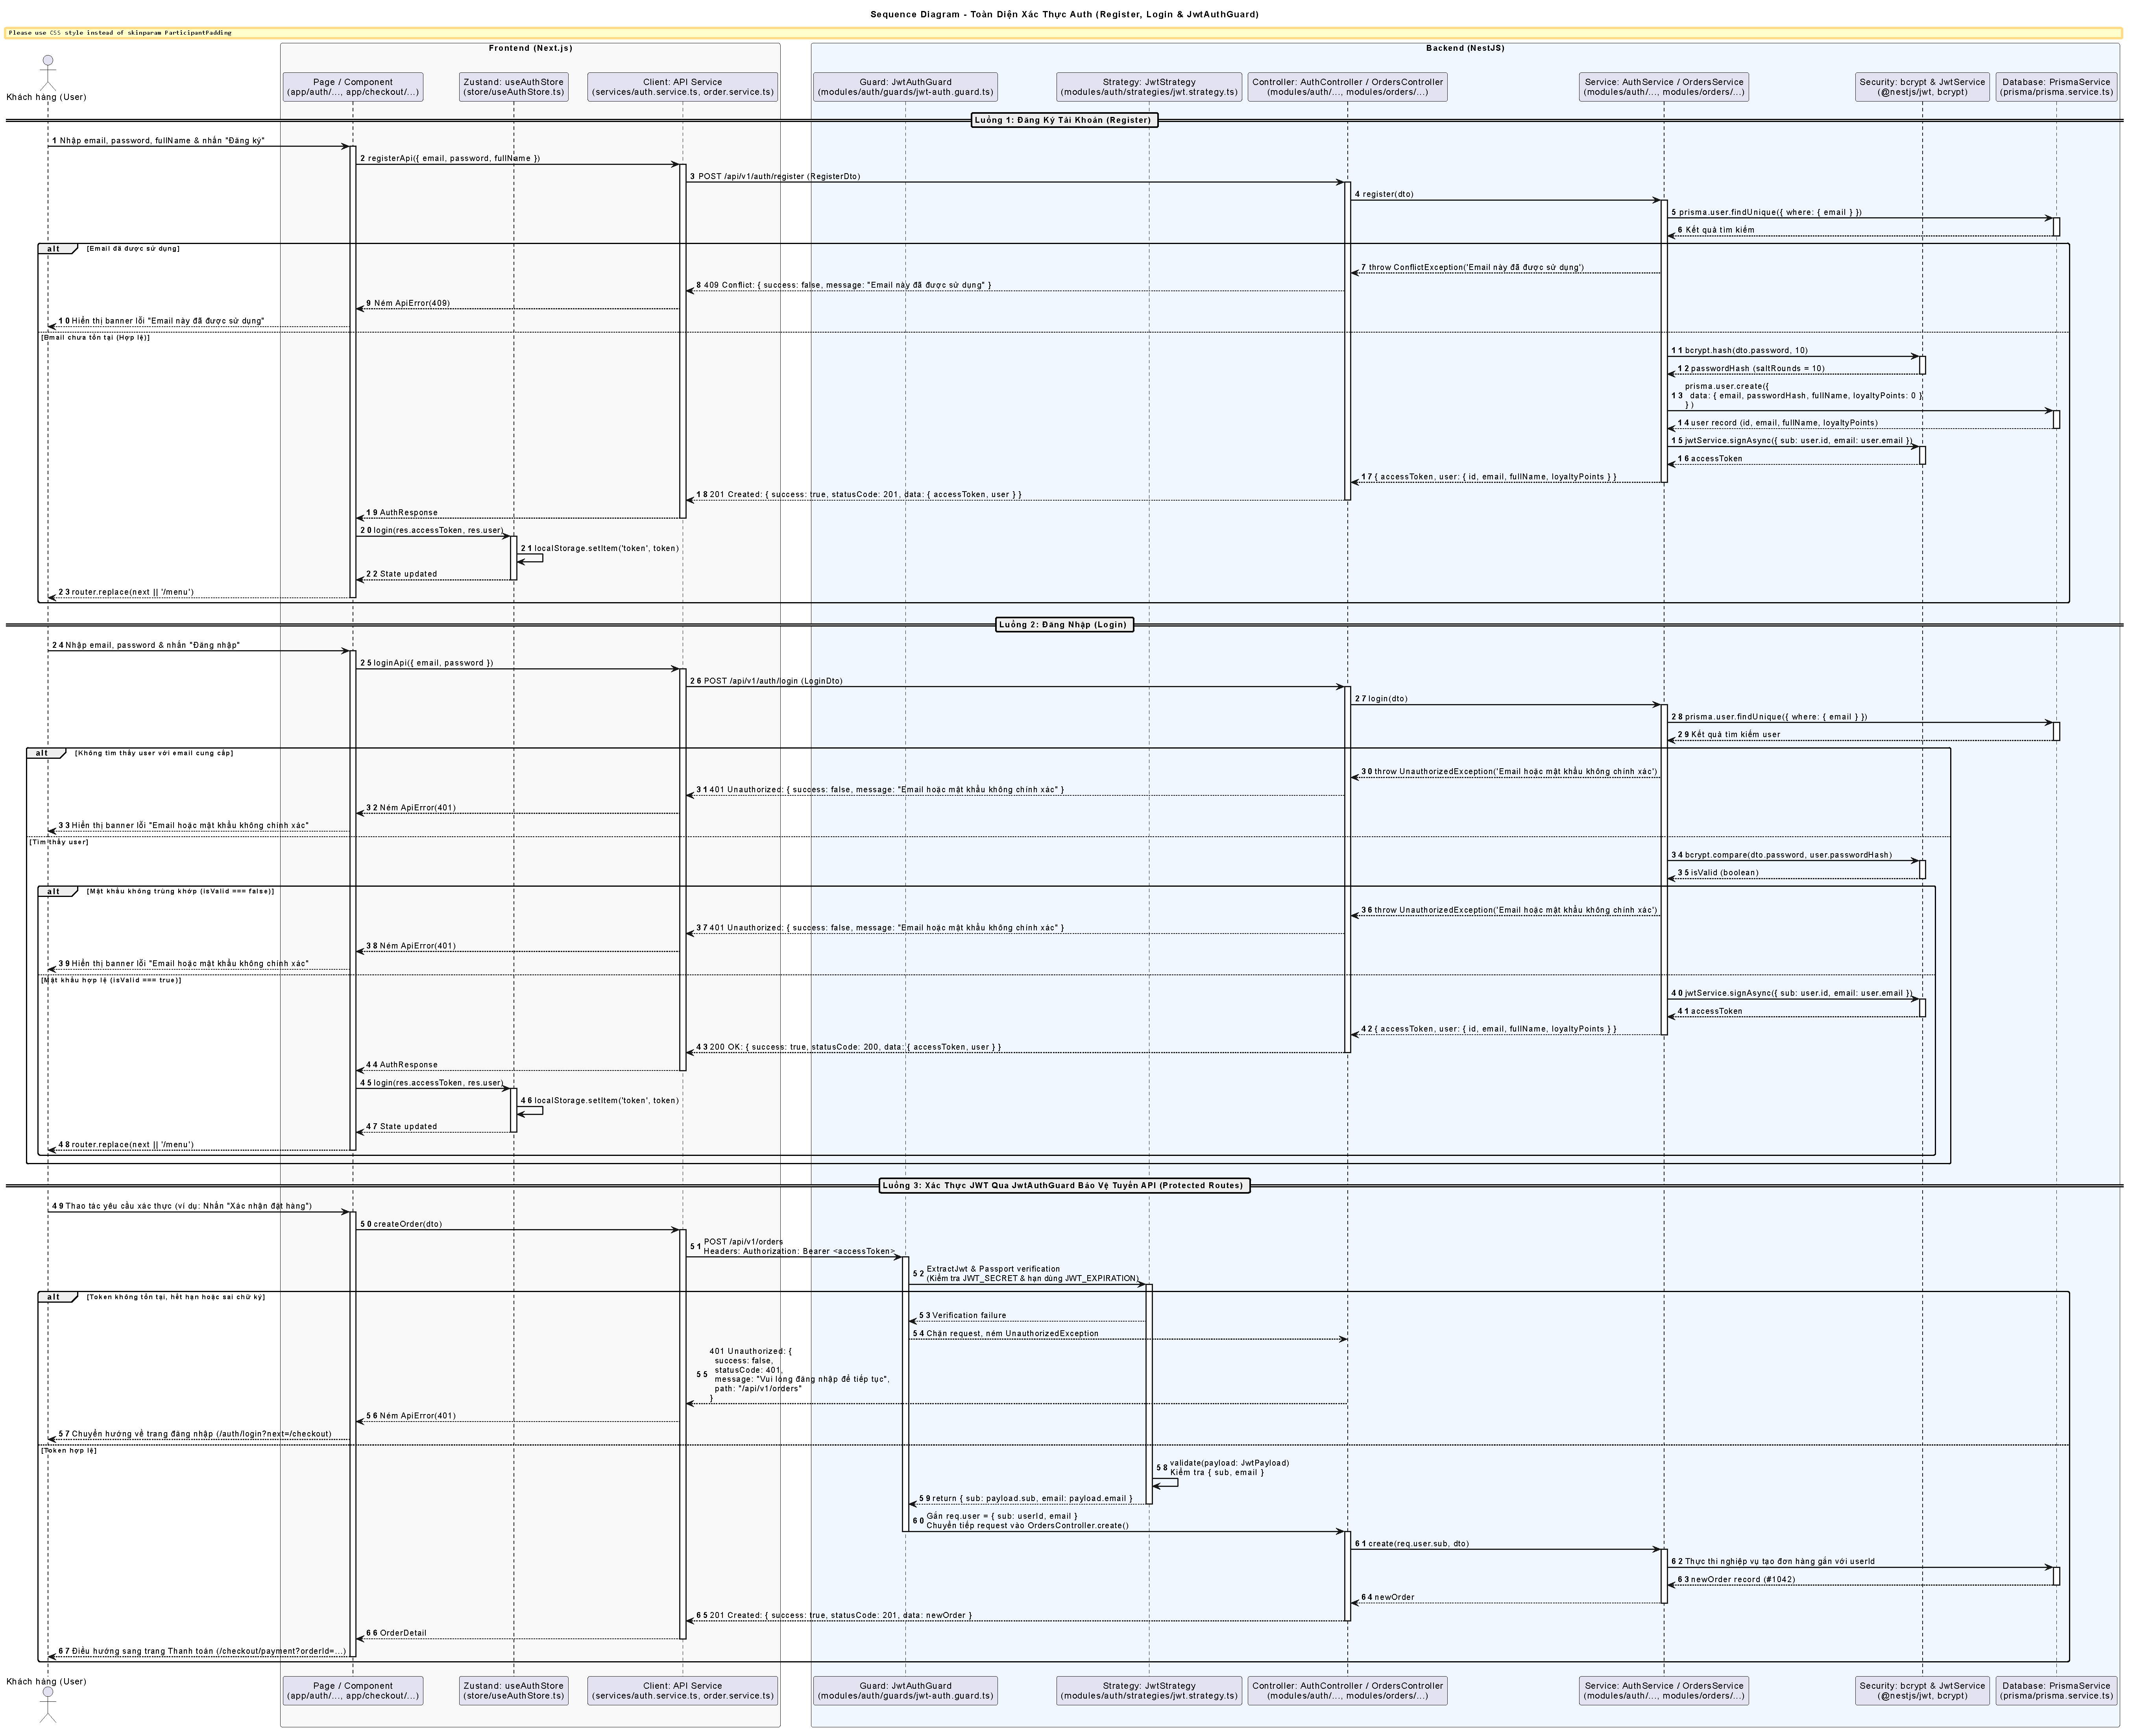
\includegraphics[width=0.9\textwidth]{figures/sequence-auth.pdf}
    \caption{Sơ đồ Tuần tự - Phân hệ Xác thực (Happy path \& Exception paths)}
    \label{fig:sequence-auth}
\end{figure}

\subsection{Hợp đồng API (API Contract)}
\begin{table}[htbp]
\centering
\small
\caption{Danh mục API Endpoints - Phân hệ Xác thực}
\label{tab:api-auth}
\begin{tabularx}{\textwidth}{llp{4cm}X}
\toprule
\textbf{Phương thức} & \textbf{Endpoint} & \textbf{Mô tả Request Body} & \textbf{Phản hồi chính} \\
\midrule
\texttt{POST} & \texttt{/api/v1/auth/register} & \texttt{\{email, password, fullName\}} (Email hợp lệ, password \(\ge 6\) ký tự) & \texttt{201 Created}: Trả về thông tin người dùng mới (loại trừ passwordHash). Lỗi: \texttt{400}, \texttt{409}. \\
\texttt{POST} & \texttt{/api/v1/auth/login} & \texttt{\{email, password\}} & \texttt{200 OK}: Trả về \texttt{accessToken} và thông tin người dùng. Lỗi: \texttt{400}, \texttt{401}. \\
\bottomrule
\end{tabularx}
\end{table}

\subsection{Ánh xạ Cơ sở dữ liệu (Database Mapping)}
Mọi thao tác của AuthModule tác động trực tiếp lên bảng \texttt{users}:
\begin{itemize}
    \item \textbf{Đăng ký:} Gọi \texttt{prisma.user.findUnique(\{ where: \{ email \} \})}. Nếu tồn tại \(\to\) throw \texttt{ConflictException}. Nếu chưa, thực thi \texttt{bcrypt.hash(password, 10)} và gọi \texttt{prisma.user.create(\{ data: \{ email, passwordHash, fullName, loyaltyPoints: 0 \} \})}.
    \item \textbf{Đăng nhập:} Gọi \texttt{prisma.user.findUnique(\{ where: \{ email \} \})}. Nếu không tìm thấy hoặc \texttt{bcrypt.compare()} trả về false \(\to\) throw \texttt{UnauthorizedException}.
    \item \textbf{Bảo mật dữ liệu:} Trường \texttt{passwordHash} tuyệt đối được lược bỏ trước khi gán vào đối tượng trả về thông qua destructuring: \texttt{const \{ passwordHash, ...userWithoutPassword \} = user}.
\end{itemize}

\subsection{Kịch bản Kiểm thử (Test Cases)}
\begin{table}[htbp]
\centering
\small
\caption{Tóm lược các Ca kiểm thử tiêu biểu - Phân hệ Xác thực}
\label{tab:tc-auth}
\begin{tabularx}{\textwidth}{llp{2.6cm}p{3cm}Xc}
\toprule
\textbf{Mã TC} & \textbf{Loại} & \textbf{Tiền điều kiện} & \textbf{Endpoint / Màn hình} & \textbf{Kết quả mong đợi} & \textbf{Trạng thái} \\
\midrule
\texttt{TC-AUTH-API-01} & Hợp lệ & Email chưa tồn tại & \texttt{POST /auth/register} & HTTP 201, tạo user mới, băm bcrypt 10 rounds & Chưa chạy \\
\texttt{TC-AUTH-API-03} & Lỗi & Email đã tồn tại & \texttt{POST /auth/register} & HTTP 409, message "Email đã được sử dụng" & Chưa chạy \\
\texttt{TC-AUTH-API-05} & Hợp lệ & Đã có tài khoản & \texttt{POST /auth/login} & HTTP 200, cấp JWT accessToken & Chưa chạy \\
\texttt{TC-AUTH-API-07} & Lỗi & Mật khẩu không đúng & \texttt{POST /auth/login} & HTTP 401, message "Email hoặc mật khẩu không chính xác" & Chưa chạy \\
\texttt{TC-AUTH-UI-01} & Giao diện & Đang ở trang \texttt{/login} & Màn hình Đăng nhập & Hiển thị form, nút "Đăng nhập", chuyển hướng thành công & Chưa chạy \\
\bottomrule
\end{tabularx}
\end{table}

\subsection{Giao diện Người dùng}
\begin{figure}[htbp]
    \centering
    \begin{subfigure}[b]{0.48\textwidth}
        \centering
        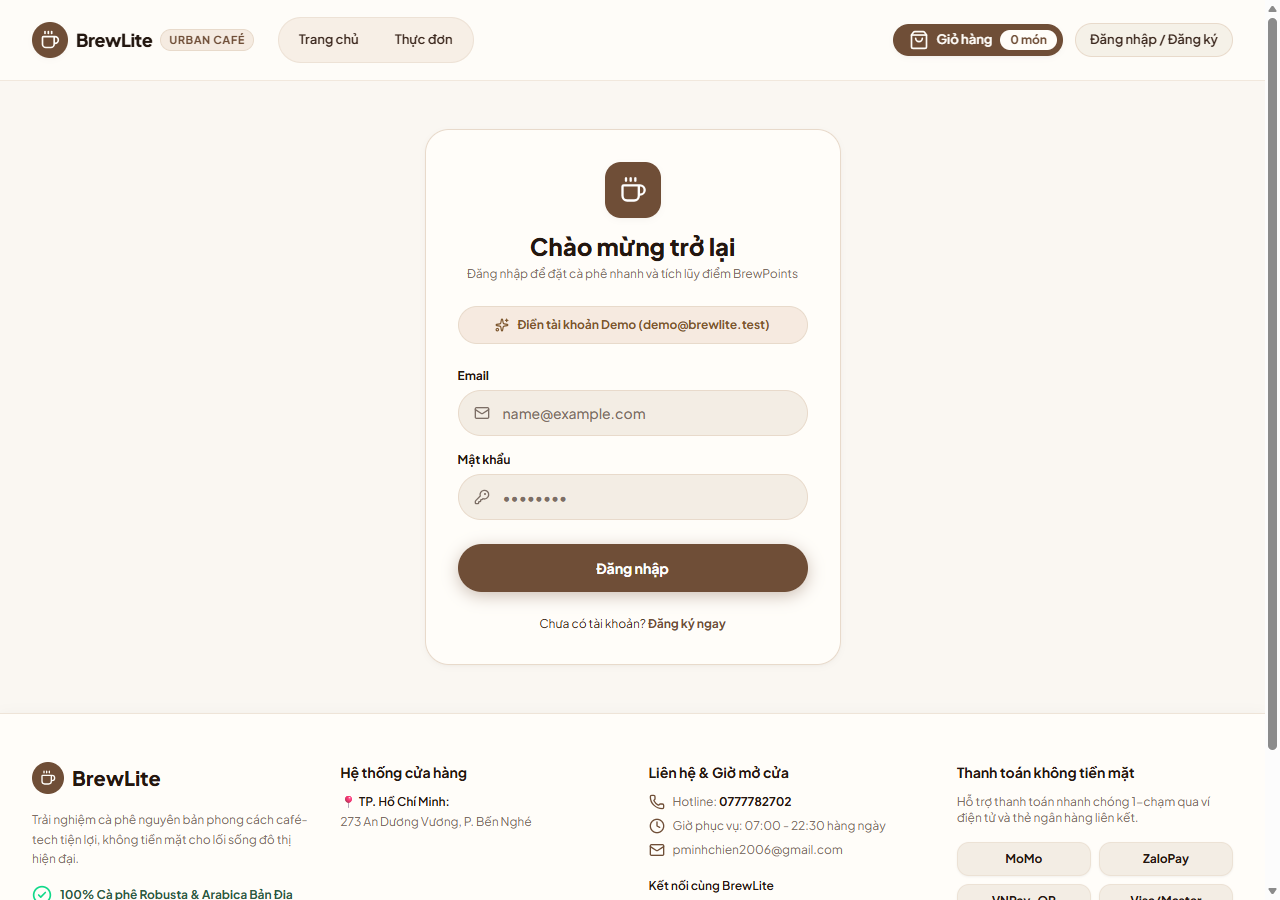
\includegraphics[width=\textwidth]{figures/ui-auth-login.png}
        \caption{Màn hình Đăng nhập}
        \label{fig:ui-auth-login}
    \end{subfigure}
    \hfill
    \begin{subfigure}[b]{0.48\textwidth}
        \centering
        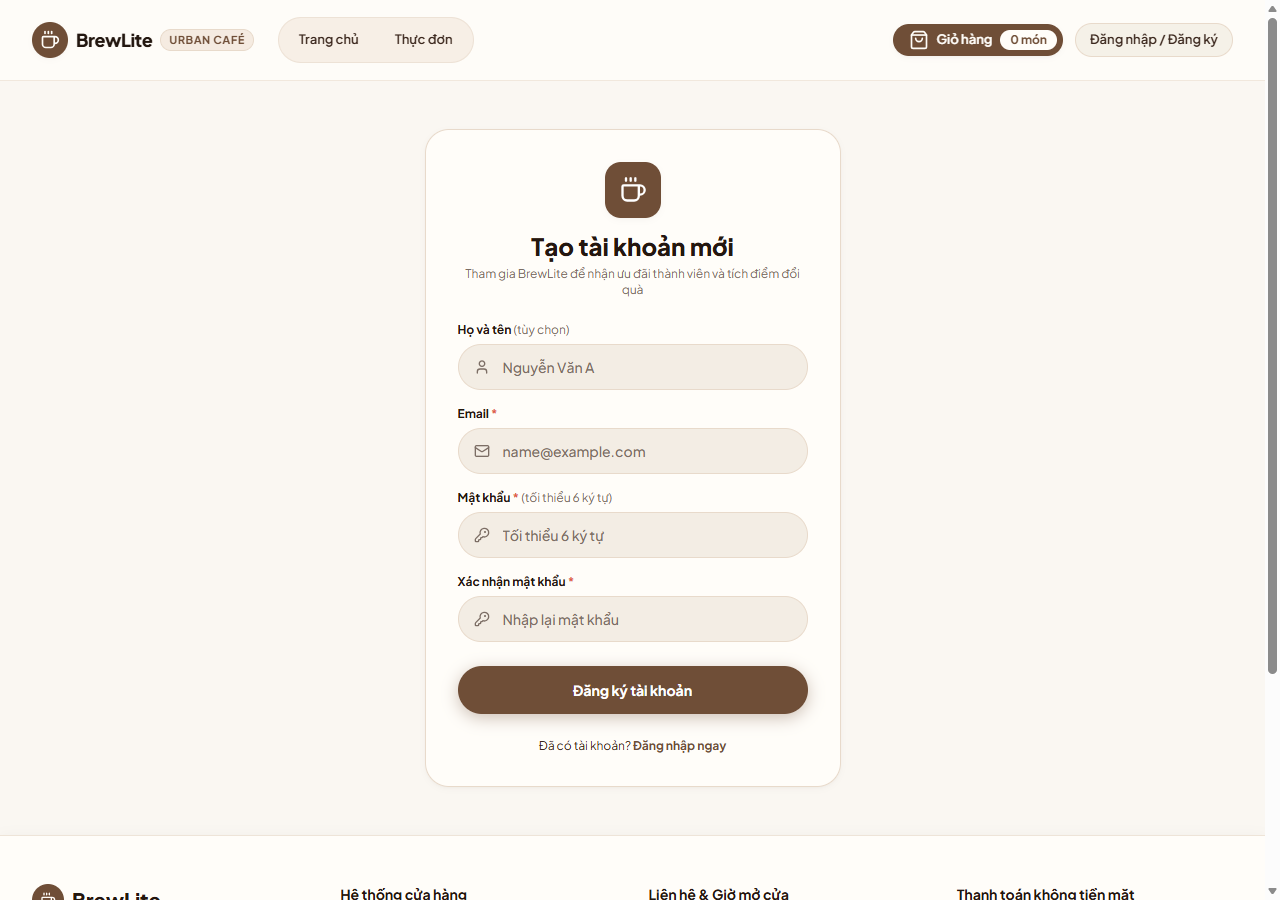
\includegraphics[width=\textwidth]{figures/ui-auth-register.png}
        \caption{Màn hình Đăng ký tài khoản}
        \label{fig:ui-auth-register}
    \end{subfigure}
    \caption{Giao diện Đăng nhập và Đăng ký người dùng}
    \label{fig:ui-auth}
\end{figure}
